\chapter{Suggested work}
\setlength{\parskip}{2.5ex plus .4ex minus .4ex}
\section{Robot Operating System}\label{sec:ROS}
The ROS\footnote{Robot Operating System} is an open source flexible framework for writing robot software. It is a collection of tools, libraries, and conventions that aim to simplify the task of creating complex and robust robot behavior across a wide variety of robotic platforms.\\
%ROS make possible to manage a robot as SIGVerse do but there is advantages to using ROS. Indeed, ROS is designed to be as distributed and modular as possible so, it encourages the collaboration to develop robot software whereas SIGVerse is not.\\
%ROS provides more than 3,000 packages and integration points for services like hardware drivers, useful external librairies,... So, everything possible with SIGVerse would be though ROS.\\
%Moreover, ROS use URDF\footnote{Unified Robot Description Format} for describing agents, which consists of an XML document like the agent description on SIGVerse.\\
At the lowest level, ROS is commonly referred to as a middleware. It provides some facilities like publishing/subscribing anonymous message passing and request/response remote procedure calls. We can see in the figure~\ref{fig:concept_de_base_ROS} the base concept of ROS. Each entity is a node who can publish or subscribe to a topic. If a node publish to a topic, every node who subscribed to it will receive the message. Many nodes can publish in the same topic and many nodes can subscribe to the same topic. Every node can publish and/or subscribe to several nodes.\\
We can also see a service between two nodes, the first node can send a request with zero or more parameters to the other node who will act and respond with parameters.

\noindent\begin{minipage}{\linewidth}% to keep image and caption on one page
\makebox[\linewidth]{%        to center the image
  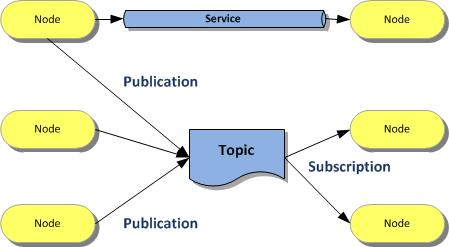
\includegraphics [width=140mm]{images/Concepts-de-base-ROS.jpg}}
\captionof{figure}{Publish/Subscribe system}\label{fig:concept_de_base_ROS}%      only if needed  
\end{minipage}

%Moreover, respect to the ROS alternatives like Mobile Robot Programming Toolkit, Microsoft Robotics Developer Studio or CARMEN, ROS has been choose for is big community, that will increase the number of users.\\

\section{SIGVerse architecture}
Currently, the architecture of SIGVerse is as shown figure~\ref{fig:SIGVerseSimple}.\\
On the Linux part, the server is running with the xml file where the agent is defined and the Controller.cpp where the initialisation and actions are defined.\\
On the Windows part, two things, SIGViewer which is a GUI and aim to show to the user the agent on the simulator. The services are all devices which can provide data to the server. That means the kinect, the oculus,...\\

\noindent\begin{minipage}{\linewidth}% to keep image and caption on one page
\makebox[\linewidth]{%        to center the image
  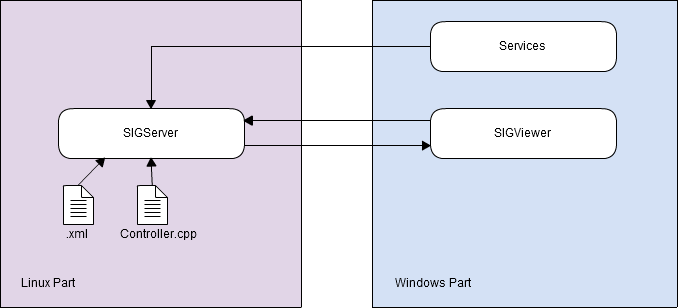
\includegraphics [width=120mm]{images/SIGVerseSimple.png}}
\captionof{figure}{SIGVerse}\label{fig:SIGVerseSimple}%      only if needed  
\end{minipage}

\section{Objective}
As seen section~\ref{sec:ROS}, using ROS to create and manipulate agents on SIGVerse will be very useful. So, I have to design and develop an interface between SIGVerse and ROS.\\
This interface has to make available the all fonctionnalities of SIGVerse from ROS, that means initializing one or more agents, make them act and make the services working though ROS.\\
The agents can be : robot, human or object.\\
The expected architecture is shown figure~\ref{fig:SIGVerseROS}. We can see the SIGServer and the ``Controller'' inside the ROS interface, that means the user will not need to interact with SIGVerse, he only defined the agent in the xml file and then, interacting with ROS, send messages to the server though the interface. The user will not need to write the ``Controller'', it will be automatically generated.\\
This is an example with one xml file and one controller, but it will be necessary to generalise it to more than one.

\noindent\begin{minipage}{\linewidth}% to keep image and caption on one page
\makebox[\linewidth]{%        to center the image
  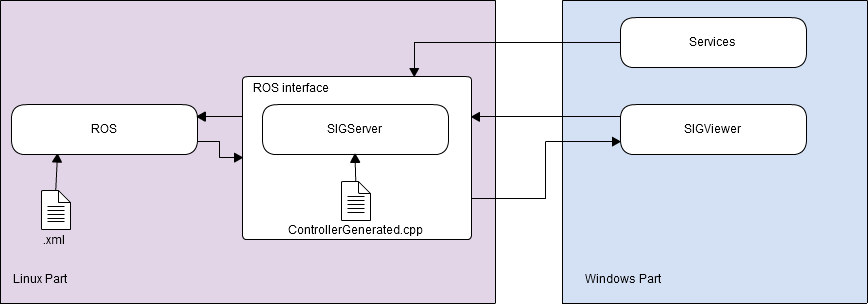
\includegraphics [width=150mm]{images/SIGVerseROS.png}}
\captionof{figure}{SIGVerse with ROS interface}\label{fig:SIGVerseROS}%      only if needed  
\end{minipage}

\section{Fonctionalities requiered}
\subsection{General requierement} %Besoins généraux
Currently, SIGVerse has two parts: SIGServer and SIGViewer and they communicate directly together as seen figure~\ref{fig:SIGVerseSimple}.\\
The aim is to find a way for the ROS users for using SIGVerse. That means the ROS user will only write ROS code and this will be enough for manipulate the simulator.\\
Right now, if the ROS user wants to do it, he has to make the interface himself, mapping the SIGVerse function which is needed. That is why, a common interface with the main functions are useful. After that, the user will have the possibility to enhance it.\\

Three agents are available on SIGVerse: the robot, the human and the object and different actions are available for each one. But some same actions are available for many of them. Indead the robot agent inherit from the object agent and the human can be a special robot.

\subsection{Use case}
The main use case is for the Robocup competition. Indeed, with this interface, ROS users could participate to the competition.\\
RoboCup is an annual international robotics competition founded in 1997.\\
There are many stages of competition, RoboCupRescue, RoboCup@Home, RoboCupJunior,...\\
The best known is the football competition where two team of robots are playing football, but the Inamura lab works on RoboCup@Home using SIGVerse. Three kinds of task are competing, the clean up task, the follow me and the EGPSR task.\\
In a simple clean up task, the robot detects the trash, go to take it and puts it in the trashbox detected. Points are given for every good things done like ``take the trash'' and ``put it in the trashbox'', but points are removed if a collision occurs.\\
The aim of the follow me task is to follow someone without collision, don't lose him and knowing in which direction after entering the elevator. Indeed, if the man entry the elevator, the robot will enter too but the man will not be able to go out before the robot do it.\\
The EGPSR task is the interaction between the human and the robot. The man asks the robot for an object in a room and the robot has to go to the right room and get it back.\\
First of all, the clean up task has to work with ROS, that means the methods used with the robot and some methods of objects.\\
After that, there is a third agent, the human, so the follow up task will be a pertinent example.
 

\section{ROS and SIGVerse}
On SIGVerse an agent is defined by an XML file for his representation and a ``controller'' for his dynamic. The dynamic allows an agent to act, receive message or send message.\\
Currently, the user has to transform the ``Controller'' into a ROS node himself, defining the interface for each method needed.\\
We can see in figure~\ref{fig:sig_ros} an example. Indeed, we can see the ``Controller'' inside the server who is also a ROS node. That is why it can publish a message to a topic and subscribe to ``Velocity Topic''. After that, any ROS node can be created and publish or subscribe to topics, the SIGVerse agent can receive instructions from a topic or a service.\\

In this example figure~\ref{fig:sig_ros} given on the SIGVerse wiki page\cite{SIGVerseWikiROS}, the ``Controller'' launch the ROS node when the simulation starts and the topics are created. However, we want the user to write only ROS code and do not bother himself with the ``Controller'' and SIGVerse functioning.
\noindent\begin{minipage}{\linewidth}% to keep image and caption on one page
\makebox[\linewidth]{%        to center the image
  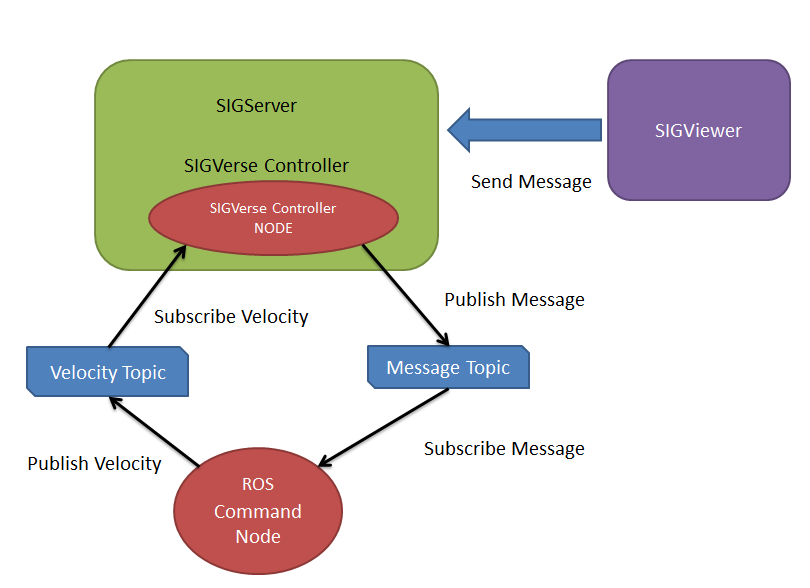
\includegraphics [width=150mm]{images/sig_ros.png}}
\captionof{figure}{SIGVerse controller sending and receiving message}\label{fig:sig_ros}%      only if needed  
\end{minipage}

%L'objectif est de pouvoir modéliser en spécifiant au sein d'un système dynamique des populations d'individus.\\
%Un individu est formalisé par un système d'équations différentielles et tous les individus d'une population se réfèrent au même système d'équations différentielles.\\
%Au sein d'une population les individus peuvent différer de par la valeur de leurs paramètres mais ce n'est pas une obligation.\\
%\\
%La dynamique des populations est définie par un ensemble d’événements portant sur les individus. Un évènement est défini par des conditions d'activation et des effets.\\
%Les conditions d'activation sont exprimées en fonction du temps de la simulation ou de l'état du système simulé. L'état du système est l'union de tous les états des individus.\\
%Il existe 3 types d'effet: Création d'un individu, suppression d'un individu et réinitialisation d'un individu.

%\subsection{Structure du modèle DEVS}
%Chaque individu est un système d'équations différentielles défini par une classe C++. Cette classe est appelée classe d'individu. C'est elle qui doit être défini par l'utilisateur puis qui servira de base pour créer tous les individus de ce type là. C'est pourquoi chaque individu de même type, a la même dynamique, seuls les paramètres peuvent varier entre eux si l'utilisateur souhaite en modifier un ou plusieurs.\\
%Chaque individu est indépendant, ils n'intéragissent pas directement les un avec les autres. Ils doivent communiquer par l'intermédiaire d'un même controleur auquels ils sont tous connectés.\\
%Chaque port de sortie de chaque individu est relié aux ports d'entrée du controleur, ce qui permet à ce dernier de recevoir des évènements, les traiter et envoyer des réponses adéquates par l'intermédiaire de ses ports de sortie reliés à chaque individu par des ports d'entrée.\\
%Lors de la simulation, la dynamique du controleur se met en marche. Elle initialise tous les individus, exécute sa dynamique interne, reçoit les évènements externes et envoie des réponses aux individus. Durant la simulation, le controleur peut à tout moment, créer un nouvel individu, en supprimer ou en modifier les paramètres grâces aux évènements qu'il reçoit en entrée et qu'il peut envoyer en sortie.\\
%Par exemple :\\
%\noindent\begin{minipage}{\linewidth}% to keep image and caption on one page
%\makebox[\linewidth]{%        to center the image
%  \includegraphics [width=150mm]{images/exemple_ibm.png}}
%\captionof{figure}{Trois Loups créés par le controleur lors de la simulation}%\label{visina8}%      only if needed  
%\end{minipage}

%Le controleur crée les individus ``Loup 1'', ``Loup 2'' et ``Loup 3'' qui sont bien indépendants les uns des autres et tous reliés au controleur comme expliqué au paragraphe précédent. \\
%
%\subsection{IBM dans VLE}
%Dans VLE, chaque système ou simulation est représenté par un Vpz qui est un fichier xml où est décrit tout le système. Modèles présents (individus), conditions expérimentales (valeurs des paramètres), classes d'individus, ports d'entrées et de sorties...\\
%Dans le Vpz, un controleur est obligatoirement présent s'il s'agit d'un système IBM. Il se crée automatiquement lors de la première ouverture du plugin IBM. \\Ensuite, les modèles souhaités par l'utilisateur sont créés lors de la simulation par le controleur grâce aux classes d'individu définies dans le vpz.\\
%Par exemple : \\
%\noindent\begin{minipage}{\linewidth}% to keep image and caption on one page
%\makebox[\linewidth]{%        to center the image
%  \includegraphics [width=160mm]{images/vpz1.png}}
%\captionof{figure}{Composition d'un Vpz}%\label{visina8}%      only if needed  
%\end{minipage}
%
%Ici, le controleur crée n Loups et m Moutons lors de la simulation, mais seul le modèle ``Controleur'' est présent dans le vpz. Le controleur est cependant lié aux classes ``Loup'' et ``Mouton'' afin de pouvoir créer les individus.

%\section{Fonctionnalités du plugin}
%À son ouverture, le plugin récupère toutes les classes d'individu déjà présentes dans le Vpz. Il offre ensuite la possibilité d'ouvrir le plugin Forrester afin de créer d'autres classes et modifier ou supprimer les classes existantes.\\
%Afin de manipuler les individus lors de la simulation, le plugin propose un champs de texte afin que l'utilisateur exprime ces besoins par l'intermédiare d'un petit langage simple appelé Lua et quelques extensions que j'aurai développées.\\
%Ces besoins peuvent être multiple, ils peuvent avoir un effet sur les individus, création, suppression, modification ou bien renvoyer des informations, valeur d'une variable, nombre d'individus, identifiant d'un individu...\\
%D'autre part, le plugin crée automatiquement un exécutive appelé ``Controleur'' à son ouverture. Controleur qui sera chargé de manipuler les individus selon le script qu'aura écrit l'utilisateur, et la dynamique DEVS.\\